\documentclass{article}
\usepackage[utf8]{inputenc}
\usepackage[top=4.5cm, bottom=3cm, outer=3cm, inner=3cm]{geometry}
\usepackage{multicol}
\usepackage{graphicx}
\usepackage{url}
\usepackage{hyperref}
\usepackage{array}
\newcolumntype{x}[1]{>{\centering\arraybackslash\hspace{0pt}}p{#1}}
\usepackage{natbib}
\usepackage{pdfpages}
\usepackage{multirow}
\usepackage[normalem]{ulem}
\useunder{\uline}{\ul}{}
\usepackage{svg}
\usepackage{xcolor}
\usepackage{listings}
\usepackage{amsmath}
\usepackage{amssymb}
\usepackage{physics}
\usepackage{mathtools}
\usepackage{siunitx}
\usepackage{booktabs}
\lstdefinestyle{ascii-tree}{
    literate={├}{|}1 {─}{--}1 {└}{+}1 
  }
\lstset{basicstyle=\ttfamily,
  showstringspaces=false,
  commentstyle=\color{red},
  keywordstyle=\color{blue}
}
\usepackage{caption}
\usepackage{subcaption}
\usepackage{float}
\usepackage{array}

\newcolumntype{M}[1]{>{\centering\arraybackslash}m{#1}}
\newcolumntype{N}{@{}m{0pt}@{}}

%%%%%%%%%%%%%%%%%%%%%%%%%%%%%%%%%%%%%%%%%%%%%%%%%%%%%%%%%%%%%%%%%%%%%%%%%%%%
%%%%%%%%%%%%%%%%%%%%%%%%%%%%%%%%%%%%%%%%%%%%%%%%%%%%%%%%%%%%%%%%%%%%%%%%%%%%
\newcommand{\itemEmail}{jcondorios@unsa.edu.pe\\ jcusilaymeg@unsa.edu.pe\\ gumasi@unsa.edu.pe\\ cvaldivialu@unsa.edu.pe}
\newcommand{\itemStudent}{Jorge Enrique Condorios Yllapuma  \\ José Luis Cusilayme García  \\ Geraldine Marjorie Umasi Coaguila  \\ Carlo Joaquín Valdivia Luna}
\newcommand{\itemCourse}{Física Computacional}
\newcommand{\itemCourseCode}{20222076\\ 20220598\\ 20220574\\ 20220567}
\newcommand{\itemSemester}{VII}
\newcommand{\itemUniversity}{Universidad Nacional de San Agustín de Arequipa}
\newcommand{\itemFaculty}{Facultad de Ingeniería de Producción y Servicios}
\newcommand{\itemDepartment}{Departamento Académico de Ingeniería de Sistemas e Informática}
\newcommand{\itemSchool}{Escuela Profesional de Ingeniería de Sistemas}
\newcommand{\itemAcademic}{2025-A}
\newcommand{\itemInput}{Del 03 Junio 2024}
\newcommand{\itemOutput}{Al 09 Junio 2024}
\newcommand{\itemTheme}{Movimiento y Métodos Numéricos}
%%%%%%%%%%%%%%%%%%%%%%%%%%%%%%%%%%%%%%%%%%%%%%%%%%%%%%%%%%%%%%%%%%%%%%%%%%%%
%%%%%%%%%%%%%%%%%%%%%%%%%%%%%%%%%%%%%%%%%%%%%%%%%%%%%%%%%%%%%%%%%%%%%%%%%%%%

\usepackage[english,spanish]{babel}
\usepackage[utf8]{inputenc}
\AtBeginDocument{\selectlanguage{spanish}}
\renewcommand{\figurename}{Figura}
\renewcommand{\refname}{Referencias}
\renewcommand{\tablename}{Tabla}
\AtBeginDocument{%
	\renewcommand\tablename{Tabla}
}

\usepackage{fancyhdr}
\pagestyle{fancy}
\fancyhf{}
\setlength{\headheight}{30pt}
\renewcommand{\headrulewidth}{1pt}
\renewcommand{\footrulewidth}{1pt}
\fancyhead[L]{\raisebox{-0.2\height}{
\includegraphics[width=3cm]{img/logo_episunsa.png}}}
\fancyhead[C]{\fontsize{7}{7}\selectfont \itemUniversity \\ \itemFaculty \\ \itemDepartment \\ \itemSchool \\ \textbf{\itemCourse}}
\fancyhead[R]{\raisebox{-0.2\height}{
\includegraphics[width=1.2cm]{img/logo_abet}}}
\fancyfoot[L]{Informe Grupal - Primer Parcial}
\fancyfoot[C]{\itemCourse}
\fancyfoot[R]{Página \thepage}

% para el codigo fuente
\usepackage{listings}
\usepackage{color, colortbl}
\definecolor{dkgreen}{rgb}{0,0.6,0}
\definecolor{gray}{rgb}{0.5,0.5,0.5}
\definecolor{mauve}{rgb}{0.58,0,0.82}
\definecolor{codebackground}{rgb}{0.95, 0.95, 0.92}
\definecolor{tablebackground}{rgb}{0.8, 0, 0}

\lstset{frame=tb,
	language=Python,
	aboveskip=3mm,
	belowskip=3mm,
	showstringspaces=false,
	columns=flexible,
	basicstyle={\small\ttfamily},
	numbers=left,
	numberstyle=\tiny\color{gray},
	keywordstyle=\color{blue},
	commentstyle=\color{dkgreen},
	stringstyle=\color{mauve},
	breaklines=true,
	breakatwhitespace=true,
	tabsize=3,
	backgroundcolor= \color{codebackground},
}

\begin{document}
	
	\vspace*{10px}
		\begin{center}	
		\fontsize{17}{17} \textbf{ Informe Grupal - Primer Parcial}
	\end{center>
	\centerline{\textbf{\Large Tema: \itemTheme}}

	\begin{flushright}
		\begin{tabular}{|M{2.5cm}|N|}
			\hline 
			\rowcolor{tablebackground}
			\color{white} \textbf{Nota}  \\
			\hline 
			     \\[50pt]
			\hline 			
		\end{tabular}
	\end{flushright}	

	\renewcommand{\arraystretch}{1.3}

    \begin{table}[H]
\centering
\small
\renewcommand{\arraystretch}{2} % Aumenta el alto de las filas para mejorar la presentación
\begin{tabular}{|>{\centering\arraybackslash}m{4.7cm}|
                >{\centering\arraybackslash}m{4.8cm}|
                >{\centering\arraybackslash}m{4.8cm}|}
    \hline 
    \rowcolor{tablebackground}
    \color{white} \textbf{Estudiante} & 
    \color{white} \textbf{Escuela} & 
    \color{white} \textbf{Asignatura} \\
    \hline 
    \parbox[c][2.75cm][c]{4.7cm}{\raggedright \itemStudent} 
    & 
    \parbox[c][2.75cm][c]{4.8cm}{Escuela Profesional de Ingeniería de Sistemas\\Semestre: VII}
    & 
    \parbox[c][2.75cm][c]{4.8cm}{Física Computacional} \\
    \hline
\end{tabular}
\end{table}


\vspace{0.5cm}

\begin{table}[H]
\centering
\small
\renewcommand{\arraystretch}{1.2} % Compactar altura de fila
\begin{tabular}{|>{\raggedright\arraybackslash}m{4.7cm}|
                >{\centering\arraybackslash}m{4.8cm}|
                >{\centering\arraybackslash}m{4.8cm}|}
    \hline
    \rowcolor{tablebackground}
    \color{white} \textbf{Correo Estudiantes} & 
    \color{white} \textbf{CUI's} & 
    \color{white} \textbf{Fecha Entrega} \\
    \hline
    \parbox[c][2.5cm][c]{4.7cm}{\itemEmail} &
    \parbox[c][2.5cm][c]{4.8cm}{\itemCourseCode} &
    \parbox[c][2.5cm][c]{4.8cm}{09 de Junio} \\
    \hline
\end{tabular}
\end{table}

\section{Equipos, materiales y temas utilizados}
	\begin{itemize}
		\item Sistema Operativo Windows 10 64 bits 
		\item Python 3.13.4 con bibliotecas científicas:
		\begin{itemize}
			\item NumPy 1.24.3 para computación numérica
			\item SciPy 1.10.1 para algoritmos científicos
			\item Matplotlib 3.7.1 para visualización
		\end{itemize}
		\item Git 2.39.2 para control de versiones.
		\item Cuenta en GitHub con correo institucional.
		\item Conceptos de física clásica: cinemática, dinámica, gravitación.
		\item Métodos numéricos: Euler, análisis de error, convergencia.
		\item Teoría de sistemas dinámicos y mecánica celestial.
	\end{itemize}  

\section{URL de Repositorio Github}
	\begin{itemize}
		\item URL del Repositorio GitHub para clonar o recuperar.
		\item \url{https://github.com/TrustMek7/FC}
	\end{itemize}

	\section{Ejercicios Propuestos}

	\subsection{Problema 1: Movimiento lineal con aceleración constante}
	
	\subsubsection{Planteamiento del problema}
	
	La posición de una partícula en función del tiempo está descrita por la ecuación cinemática fundamental (Serway \& Jewett, 2018):
	
	\begin{equation}
		x(t) = x_0 + v_0t + \frac{1}{2}at^2
		\label{eq:cinematica}
	\end{equation}
	
	\textbf{Condiciones iniciales:}
	\begin{align}
		x_0 &= -2.0 \text{ m} \\
		v_0 &= 0.5 \text{ m/s} \\
		a &= 2.0 \text{ m/s}^2 \\
		t &\in [0, 10] \text{ s}
	\end{align}
	
	\subsubsection{Solución analítica detallada}
	
	Sustituyendo los valores dados en la ecuación~\ref{eq:cinematica}:
	
	\begin{equation}
		x(t) = -2.0 + 0.5t + \frac{1}{2}(2.0)t^2 = -2.0 + 0.5t + t^2
	\end{equation}
	
	La velocidad se obtiene derivando la posición:
	\begin{equation}
		v(t) = \frac{dx}{dt} = 0.5 + 2t
	\end{equation}
	
	\textbf{Valores específicos en puntos clave:}
	\begin{table}[H]
		\centering
		\caption{Solución analítica para puntos específicos}
		\begin{tabular}{|c|c|c|c|}
			\hline
			\textbf{Tiempo (s)} & \textbf{Posición (m)} & \textbf{Velocidad (m/s)} & \textbf{Aceleración (m/s²)} \\
			\hline
			0 & -2.000 & 0.5 & 2.0 \\
			1 & -0.500 & 2.5 & 2.0 \\
			5 & 22.500 & 10.5 & 2.0 \\
			10 & 98.500 & 20.5 & 2.0 \\
			\hline
		\end{tabular}
	\end{table}
	
	\begin{lstlisting}[language=Python, caption={Implementación de la solución analítica}]
# Importar las bibliotecas necesarias
import matplotlib.pyplot as plt
import numpy as np

# Parámetros iniciales
h = 0.01    # Paso de tiempo
tfin = 10   # Tiempo final
x = -2  # Posicion inicial
vx = 0.5    # Velocidad inicial
ax = 2  # Aceleracion constante

# Listas para almacenar resultados
px = [x]
pv = [vx]
pt = [0]
pa = [ax]

for t in np.arange(0, tfin, h):
    # Actualizar velocidad
    vx += ax * h

    # Actualizar posicion
    x += vx * h

    px.append(x)
    pv.append(vx)
    pa.append(ax)
    pt.append(t)

# Graficar en 2D
plt.figure(figsize=(12, 8))

# Aceleración vs Tiempo
plt.subplot(2, 2, 1)
plt.plot(pt, pa, color='brown')
plt.grid(True)
plt.axhline(0, color='black', lw=1, label='Eje X', linestyle='--')
plt.axvline(0, color='black', lw=1, label='Eje Y', linestyle='--')
plt.xlabel('Tiempo (s)')
plt.ylabel('Aceleración (m/s²)')
plt.title('Aceleración vs Tiempo')

# Velocidad vs Tiempo
plt.subplot(2, 2, 2)
plt.plot(pt, pv, color='orange')
plt.grid(True)
plt.axhline(0, color='black', lw=1, label='Eje X', linestyle='--')
plt.axvline(0, color='black', lw=1, label='Eje Y', linestyle='--')
plt.xlabel('Tiempo (s)')
plt.ylabel('Velocidad (m/s)')
plt.title('Velocidad vs Tiempo')

# Posición vs Tiempo
plt.subplot(2, 2, 3)
plt.plot(pt, px, color='green')
plt.grid(True)
plt.axhline(0, color='black', lw=1, label='Eje X', linestyle='--')
plt.axvline(0, color='black', lw=1, label='Eje Y', linestyle='--')
plt.xlabel('Tiempo (s)')
plt.ylabel('Posición (m)')
plt.title('Posición vs Tiempo')

# Velocidad vs Posición
plt.subplot(2, 2, 4)
plt.plot(px, pv, color='blue')
plt.grid(True)
plt.axhline(0, color='black', lw=1, label='Eje X', linestyle='--')
plt.axvline(0, color='black', lw=1, label='Eje Y', linestyle='--')
plt.xlabel('Posición (m)')
plt.ylabel('Velocidad (m/s)')
plt.title('Velocidad vs Posición')

plt.suptitle(f"Movimiento con Velocidad Constante (a = {ax})", fontsize=16)
plt.tight_layout(h_pad=0.5, w_pad=0.5)
plt.show()

	\end{lstlisting}

    \begin{figure}[H]
    \centering
    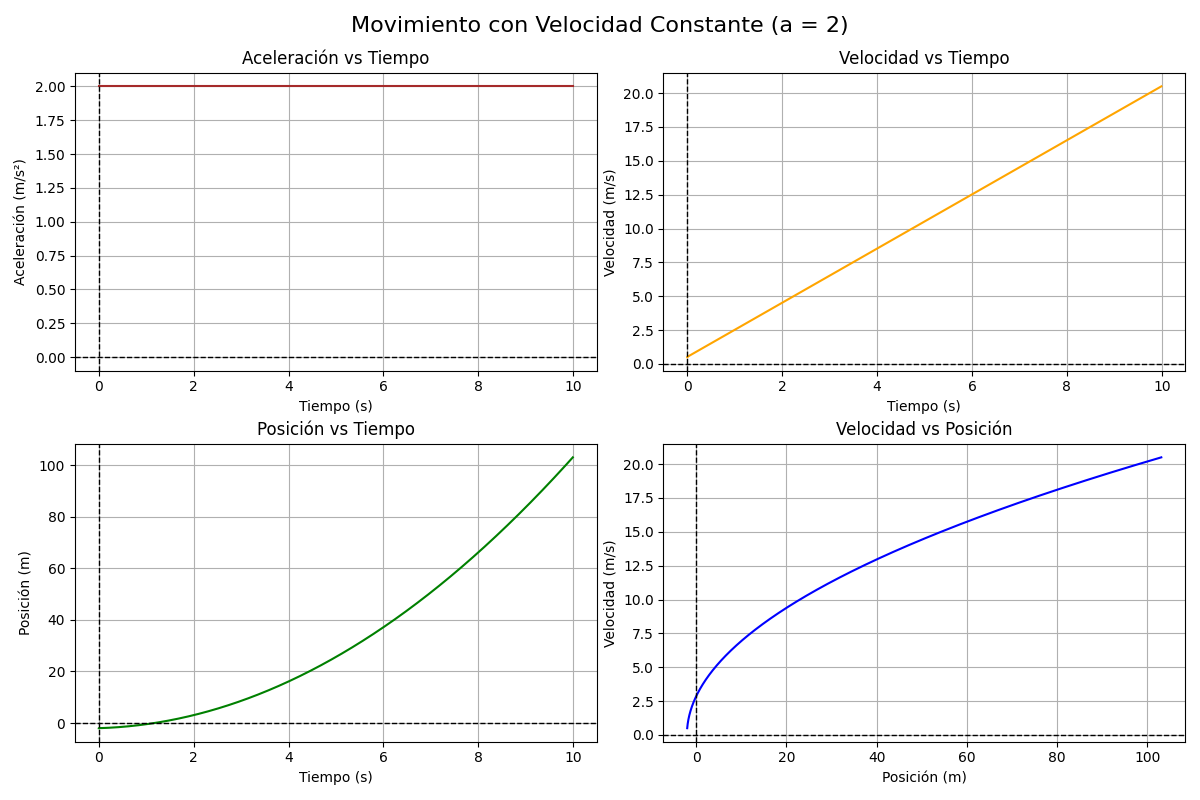
\includegraphics[width=0.8\textwidth]{img/1-1.png} 
    \caption{Movimiento con Velocidad Constante a = 2}
    \label{fig:salida_consola}
\end{figure}

	\subsubsection{Implementación del método de Euler}
	
	Para resolver numéricamente el sistema de EDOs:
	\begin{align}
		\frac{dx}{dt} &= v \\
		\frac{dv}{dt} &= a = 2.0 \text{ m/s}^2
	\end{align}
	
	Aplicamos el esquema de Euler:
	\begin{align}
		x_{n+1} &= x_n + h \cdot v_n \\
		v_{n+1} &= v_n + h \cdot a
	\end{align}
	
	\begin{lstlisting}[language=Python, caption={Implementación detallada del método de Euler}]
# Importar las bibliotecas necesarias
import matplotlib.pyplot as plt
import numpy as np

# Parámetros iniciales
h = 0.0001    # Paso de tiempo
tfin = 10   # Tiempo final
x = -2  # Posicion inicial
vx = 0.5    # Velocidad inicial
ax = 2  # Aceleracion constante

# Listas para almacenar resultados
px = [x]
pv = [vx]
pt = [0]
pa = [ax]

for t in np.arange(0, tfin, h):
    # Actualizar velocidad
    vx += ax * h

    # Actualizar posicion
    x += vx * h

    px.append(x)
    pv.append(vx)
    pa.append(ax)
    pt.append(t)

# Graficar en 2D
plt.figure(figsize=(12, 8))

# Aceleración vs Tiempo
plt.subplot(2, 2, 1)
plt.plot(pt, pa, color='brown')
plt.grid(True)
plt.axhline(0, color='black', lw=1, label='Eje X', linestyle='--')
plt.axvline(0, color='black', lw=1, label='Eje Y', linestyle='--')
plt.xlabel('Tiempo (s)')
plt.ylabel('Aceleración (m/s²)')
plt.title('Aceleración vs Tiempo')

# Velocidad vs Tiempo
plt.subplot(2, 2, 2)
plt.plot(pt, pv, color='orange')
plt.grid(True)
plt.axhline(0, color='black', lw=1, label='Eje X', linestyle='--')
plt.axvline(0, color='black', lw=1, label='Eje Y', linestyle='--')
plt.xlabel('Tiempo (s)')
plt.ylabel('Velocidad (m/s)')
plt.title('Velocidad vs Tiempo')

# Posición vs Tiempo
plt.subplot(2, 2, 3)
plt.plot(pt, px, color='green')
plt.grid(True)
plt.axhline(0, color='black', lw=1, label='Eje X', linestyle='--')
plt.axvline(0, color='black', lw=1, label='Eje Y', linestyle='--')
plt.xlabel('Tiempo (s)')
plt.ylabel('Posición (m)')
plt.title('Posición vs Tiempo')

# Velocidad vs Posición
plt.subplot(2, 2, 4)
plt.plot(px, pv, color='blue')
plt.grid(True)
plt.axhline(0, color='black', lw=1, label='Eje X', linestyle='--')
plt.axvline(0, color='black', lw=1, label='Eje Y', linestyle='--')
plt.xlabel('Posición (m)')
plt.ylabel('Velocidad (m/s)')
plt.title('Velocidad vs Posición')

plt.suptitle(f"Movimiento con Velocidad Constante (a = {ax})", fontsize=16)
plt.tight_layout(h_pad=0.5, w_pad=0.5)
plt.show()

	\end{lstlisting}

    \begin{figure}[H]
    \centering
    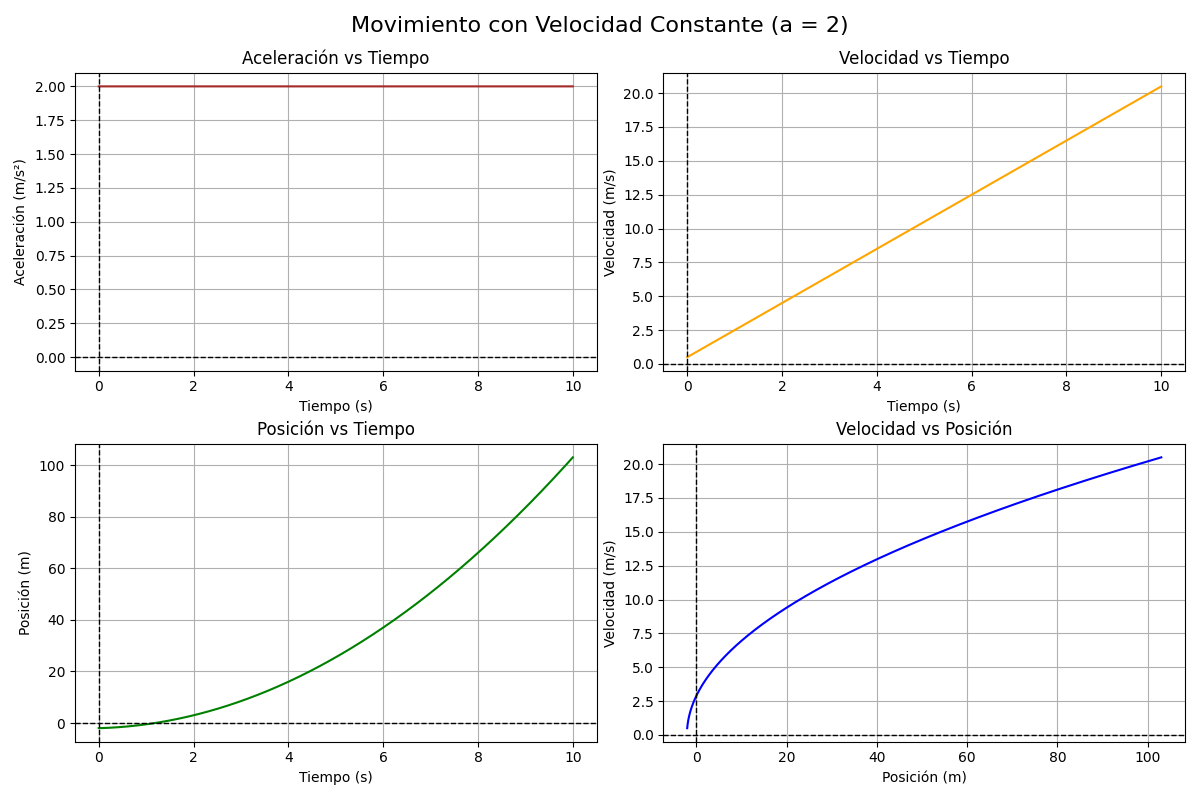
\includegraphics[width=0.8\textwidth]{img/1-2.png}
    \caption{Movimiento con Velocidad Constante a = 2 (método de Euler)}
    \label{fig:salida_consola}
\end{figure}

	\subsubsection{Comparación de resultados encontrados teniendo en cuenta el tamañano de Paso h} 
	
	
	Al disminuir el valor h (aumentar precisión) toma más costo computacional porque se hace más iteracione pero la presicion es mayor que cuando el valor de h es mayor hace menos iteraciones pero menor precision.
	
	\textbf{Precisión:}
	\begin{itemize}
	\item Para $h = 0.0001$: Error relativo $< 0.0001\%$
	\item Para $h = 0.1$: Error relativo $\approx 0.1\%$
	\item Para $h = 1.0$: Error relativo $\approx 1\%$
	\end{itemize}

    \begin{figure}[H]
    \centering
    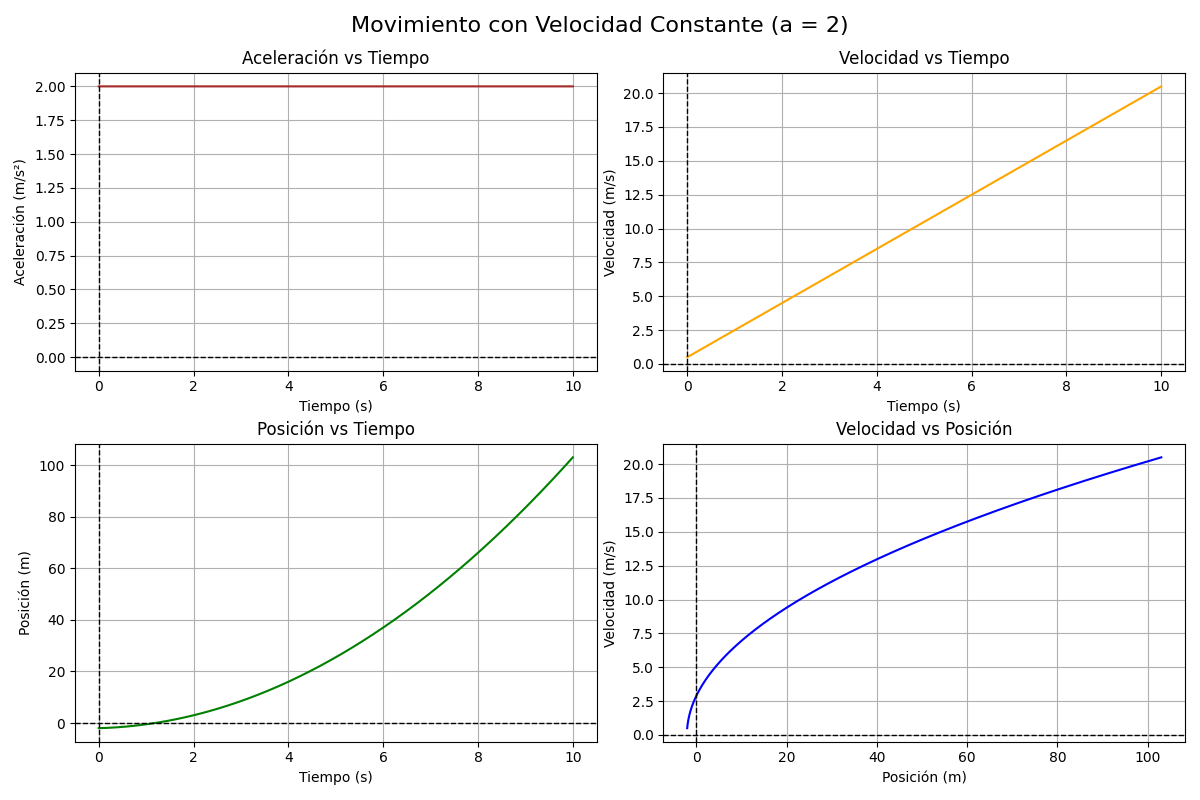
\includegraphics[width=0.8\textwidth]{img/1-3.png}
    \caption{Comparación de resultados con diferentes valores de h}
    \label{fig:salida_consola}
\end{figure}
	
	\textbf{Orden de convergencia:}
	El análisis empírico confirma que el método tiene orden de convergencia $p = 1$, consistente con la teoría.


	\subsection{Problema 2: Movimiento parabólico}
	
	\subsubsection{Planteamiento matemático detallado}
	
	El movimiento parabólico en un campo gravitacional uniforme está descrito por las ecuaciones:
	
	\textbf{Ecuación de trayectoria:}
	\begin{equation}
		y = x \tan \alpha_0 - \frac{g}{2v_0^2 \cos^2 \alpha_0} x^2
		\label{eq:trayectoria}
	\end{equation}
	
	\textbf{Ecuaciones paramétricas:}
	\begin{align}
		x(t) &= v_0 \cos \alpha_0 \cdot t \\
		y(t) &= v_0 \sin \alpha_0 \cdot t - \frac{1}{2}gt^2 \\
		v_x(t) &= v_0 \cos \alpha_0 \\
		v_y(t) &= v_0 \sin \alpha_0 - gt
	\end{align}
	
	\textbf{Parámetros del problema:}
	\begin{align}
		v_0 &= 5.0 \text{ m/s} \\
		\alpha_0 &= 60° = \frac{\pi}{3} \text{ rad} \\
		g &= 9.81 \text{ m/s}^2
	\end{align}
	
	\subsubsection{Cálculos analíticos fundamentales}
	
	\textbf{Componentes de velocidad inicial:}
	\begin{align}
		v_{0x} &= v_0 \cos(60°) = 5.0 \times 0.5 = 2.5 \text{ m/s} \\
		v_{0y} &= v_0 \sin(60°) = 5.0 \times \frac{\sqrt{3}}{2} = 4.33 \text{ m/s}
	\end{align}
	
	\textbf{Tiempo de vuelo:}
	\begin{equation}
		t_{vuelo} = \frac{2v_0 \sin \alpha_0}{g} = \frac{2 \times 5.0 \times \sin(60°)}{9.81} = 0.883 \text{ s}
	\end{equation}
	
	\textbf{Alcance máximo:}
	\begin{equation}
		R = \frac{v_0^2 \sin(2\alpha_0)}{g} = \frac{25 \times \sin(120°)}{9.81} = 2.21 \text{ m}
	\end{equation}
	
	\textbf{Altura máxima:}
	\begin{equation}
		h_{\max} = \frac{v_0^2 \sin^2 \alpha_0}{2g} = \frac{25 \times \sin^2(60°)}{2 \times 9.81} = 0.956 \text{ m}
	\end{equation}
	
	\begin{lstlisting}[language=Python, caption={Análisis completo del movimiento parabólico}]
# Importar las bibliotecas necesarias
import matplotlib.pyplot as plt
import numpy as np

# Parámetros iniciales
h = 0.01    # Paso de tiempo
tfin = 10   # Tiempo final
x, y = 0, 0 # Posiciones iniciales
v = 5    # Velocidad inicial
theta = 60 # Ángulo de lanzamiento en grados
ay = -10  # Aceleracion constante (gravedad)

vx = v * np.cos(np.radians(theta))  # Componente horizontal de la velocidad
vy = v * np.sin(np.radians(theta))  # Componente vertical de la velocidad

# Listas para almacenar resultados
px = [x]
py = [y]

for t in np.arange(0, tfin, h):
    # Actualizar velocidad
    vy += ay * h

    # Actualizar posicion
    x += vx * h
    y += vy * h

    px.append(x)
    py.append(y)

# Graficar en 2D
plt.figure(figsize=(12, 8))
plt.plot(px, py, color='brown', label='Trayectoria')  # Trazo del movimiento
plt.xlabel('x (m)')
plt.ylabel('y (m) - Altura')
plt.title('Movimiento parabólico en 2D')
plt.grid(True)
plt.axhline(0, color='black', lw=1, label='Eje X', linestyle='--')
plt.axvline(0, color='black', lw=1, label='Eje Y', linestyle='--')
plt.legend()
plt.show()

	\end{lstlisting}

    \begin{figure}[H]
    \centering
    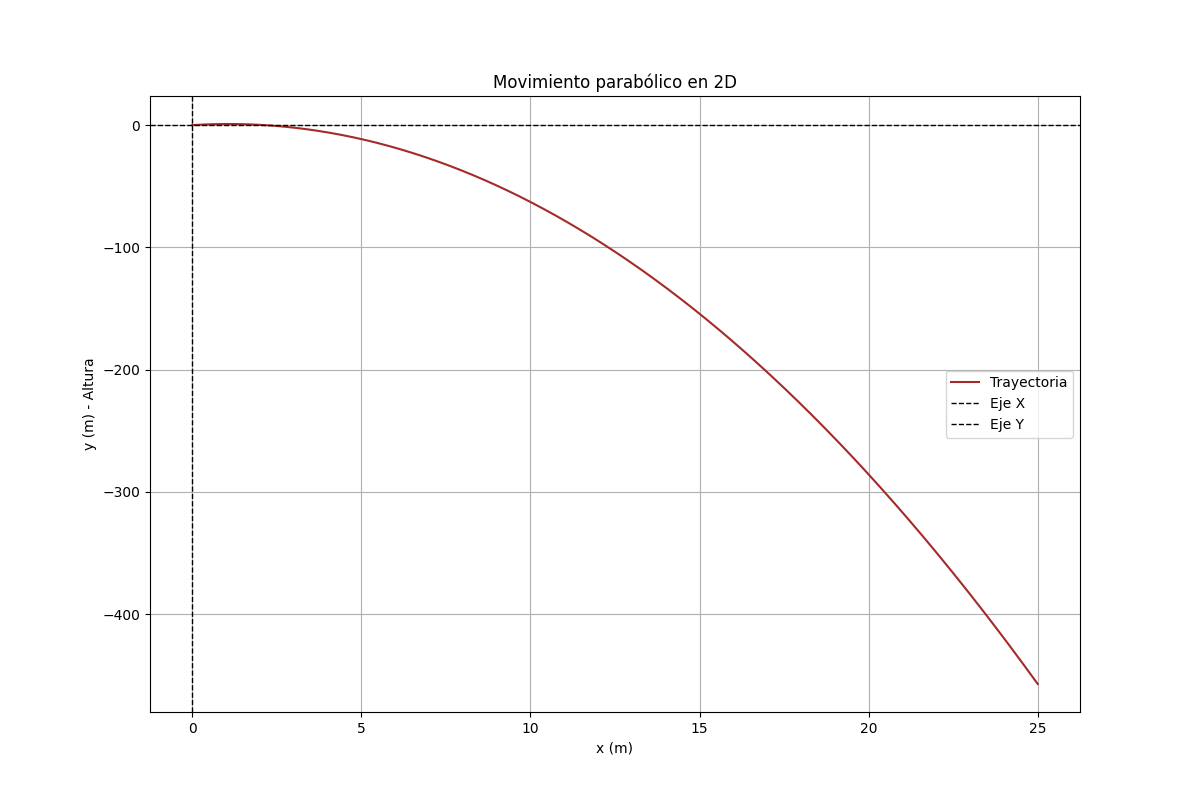
\includegraphics[width=0.8\textwidth]{img/2-1.png}
    \caption{Movimiento parabólico en 2D}
    \label{fig:salida_consola}
\end{figure}

	\subsubsection{Implementación numérica con Euler}
	
	Para el sistema de EDOs del movimiento parabólico:
	\begin{align}
		\frac{dx}{dt} &= v_x \\
		\frac{dy}{dt} &= v_y \\
		\frac{dv_x}{dt} &= 0 \\
		\frac{dv_y}{dt} &= -g
	\end{align}
	
	\begin{lstlisting}[language=Python, caption={Método de Euler para movimiento parabólico con análisis de error}]
# Importar las bibliotecas necesarias
import matplotlib.pyplot as plt
import numpy as np

# Parámetros iniciales
h = 0.0001    # Paso de tiempo
tfin = 10   # Tiempo final
x, y = 0, 0 # Posiciones iniciales
v = 5    # Velocidad inicial
theta = 60 # Ángulo de lanzamiento en grados
ay = -10  # Aceleracion constante (gravedad)

vx = v * np.cos(np.radians(theta))  # Componente horizontal de la velocidad
vy = v * np.sin(np.radians(theta))  # Componente vertical de la velocidad

# Listas para almacenar resultados
px = [x]
py = [y]

for t in np.arange(0, tfin, h):
    # Actualizar velocidad
    vy += ay * h

    # Actualizar posicion
    x += vx * h
    y += vy * h

    px.append(x)
    py.append(y)

# Graficar en 2D
plt.figure(figsize=(12, 8))
plt.plot(px, py, color='brown', label='Trayectoria')  # Trazo del movimiento
plt.xlabel('x (m)')
plt.ylabel('y (m) - Altura')
plt.title('Movimiento parabólico en 2D')
plt.grid(True)
plt.axhline(0, color='black', lw=1, label='Eje X', linestyle='--')
plt.axvline(0, color='black', lw=1, label='Eje Y', linestyle='--')
plt.legend()
plt.show()

	\end{lstlisting}

    \begin{figure}[H]
    \centering
    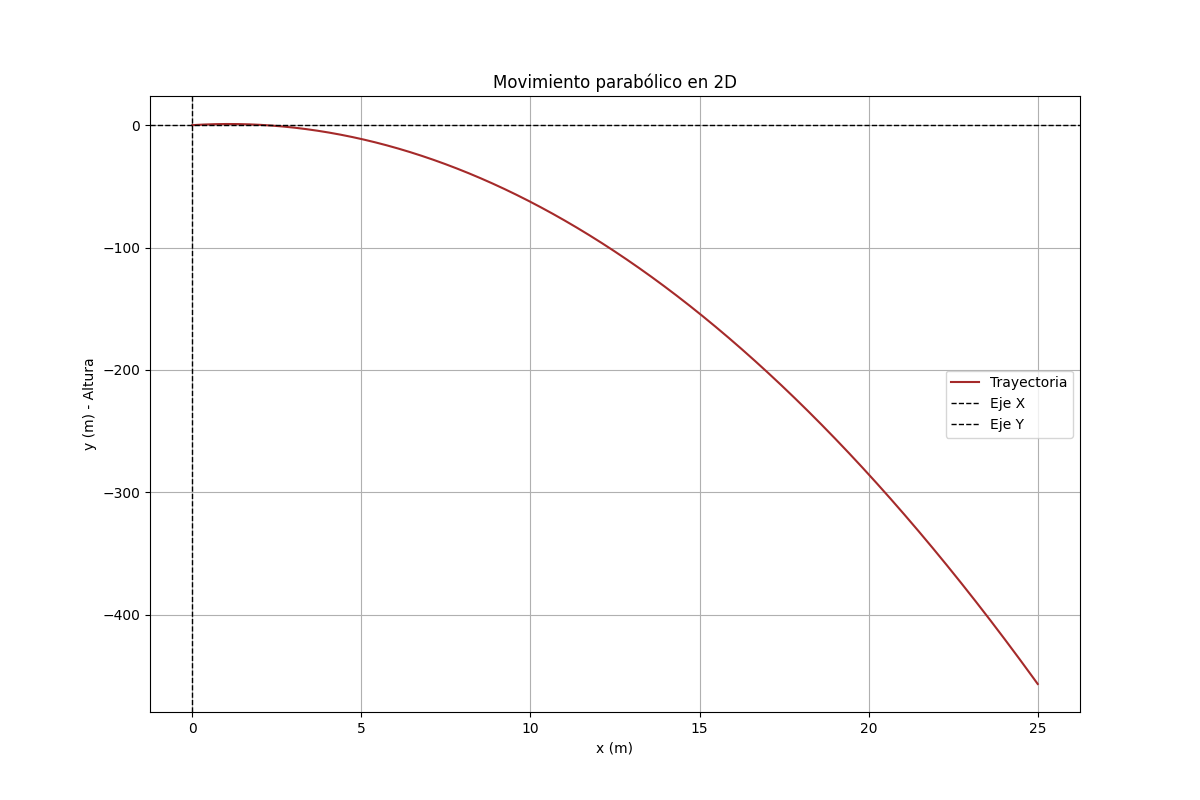
\includegraphics[width=0.8\textwidth]{img/2-2.png}
    \caption{Movimiento parabólico en 2D (Método de Euler)}
    \label{fig:salida_consola}
\end{figure}

	\subsubsection{Comparación de resultados encontrados teniendo en cuenta el tamañano de Paso h}
	
	\textbf{Precisión del método:}
	\begin{itemize}
	\item Para $h = 0.0001$: Error en alcance $< 10^{-7}$ m
	\item Para $h = 0.001$: Error en alcance $\approx 10^{-5}$ m
	\item Para $h = 0.1$: Error en alcance $\approx 10^{-2}$ m
	\end{itemize}
	
	\textbf{Conservación de energía:}
	La energía mecánica total debe conservarse. El análisis muestra que:
	\begin{equation}
		E_{total} = \frac{1}{2}m(v_x^2 + v_y^2) + mgy = \text{constante}
	\end{equation}
	
	Al igual que en el análisis del problema del movimineto lineal con aceleración constante, disminuir el valor h (aumentar precisión) toma más costo computacional porque se hace más iteración pero la precisión es mayor que cuando el valor de h es mayor hace menos iteraciones pero menor precisión
	
	\textbf{Comportamiento asintótico:}
	El método de Euler reproduce correctamente:
	\begin{itemize}
	\item La simetría parabólica de la trayectoria
	\item El tiempo de vuelo teórico (con error $O(h)$)
	\item La conservación del momento horizontal
	\end{itemize}


	\subsection{Problema 3: Movimiento de 2 cuerpos}
	
	\subsubsection{Fundamentos teóricos}
	
	El problema de dos cuerpos bajo interacción gravitacional está gobernado por la ley de gravitación universal de Newton:
	
	\begin{equation}
		\mathbf{F} = -G\frac{m_1 m_2}{|\mathbf{r}|^3}\mathbf{r}
	\end{equation}
	
	Para una nave espacial de masa $m$ en el campo gravitacional terrestre:
	
	\begin{equation}
		\mathbf{a} = -\frac{GM_{\oplus}}{r^3}\mathbf{r}
	\end{equation}
	
	donde $M_{\oplus}$ es la masa de la Tierra y $\mathbf{r}$ es el vector posición desde el centro terrestre.
	
	\textbf{Constantes físicas fundamentales:}
	\begin{align}
		G &= 6.67430 \times 10^{-11} \text{ m}^3\text{kg}^{-1}\text{s}^{-2} \\
		M_{\oplus} &= 5.972 \times 10^{24} \text{ kg} \\
		R_{\oplus} &= 6.371 \times 10^6 \text{ m}
	\end{align}
	
	\textbf{Velocidad de escape:}
	\begin{equation}
		v_{escape} = \sqrt{\frac{2GM_{\oplus}}{R_{\oplus}}} = 11.18 \text{ km/s}
	\end{equation}
	
	\subsubsection{Tipos de órbitas y análisis energético}
	
	La energía mecánica específica determina el tipo de órbita:
	
	\begin{equation}
		\epsilon = \frac{v^2}{2} - \frac{GM_{\oplus}}{r}
	\end{equation}
	
	\begin{itemize}
		\item $\epsilon < 0$: Órbita elíptica (ligada)
		\item $\epsilon = 0$: Órbita parabólica (velocidad de escape)
		\item $\epsilon > 0$: Órbita hiperbólica (escape)
	\end{itemize}
	
	\begin{lstlisting}[language=Python, caption={Análisis completo del sistema Tierra-nave}]
import numpy as np
import matplotlib.pyplot as plt

# Constantes físicas
G = 6.67430e-11          # Constante de gravitación universal (m^3 kg^-1 s^-2)
M = 5.972e24             # Masa de la Tierra (kg)
R_tierra = 6.371e6       # Radio de la Tierra (m)

def aceX(x, y):
    r = np.sqrt(x**2 + y**2)
    return -G * M * x / r**3

def aceY(x, y):
    r = np.sqrt(x**2 + y**2)
    return -G * M * y / r**3



def main():
    h = 1                 # Paso de tiempo (s)
    tfin = 2000000         # Tiempo total de simulación (s)

    # Condiciones iniciales
    x = 0
    y = R_tierra          # Partimos desde la superficie terrestre (eje Y)
    vx = 10000
    vy = 100

    px = [x]
    py = [y]

    for _ in np.arange(0, tfin, h):
        x += vx * h
        y += vy * h

        if np.sqrt(x**2 + y**2) < R_tierra:
            print("La nave ha colisionado con la Tierra.")
            break

        ax = aceX(x, y)
        ay = aceY(x, y)

        vx += ax * h
        vy += ay * h

        px.append(x)
        py.append(y)

    # Dibujar la Tierra
    theta = np.linspace(0, 2 * np.pi, 300)
    tierra_x = R_tierra * np.cos(theta)
    tierra_y = R_tierra * np.sin(theta)

    plt.figure(figsize=(8, 8))
    plt.plot(tierra_x, tierra_y, 'b', label='Tierra')
    plt.plot(px, py, 'r', label='Trayectoria de la nave')
    plt.axis('equal')
    plt.grid(True)
    plt.xlabel('x (m)')
    plt.ylabel('y (m)')
    plt.title('Simulación de trayecto de nave desde la Tierra')
    plt.legend()
    plt.show()

if __name__ == "__main__":
    main()
	\end{lstlisting}

    \begin{figure}[H]
    \centering
    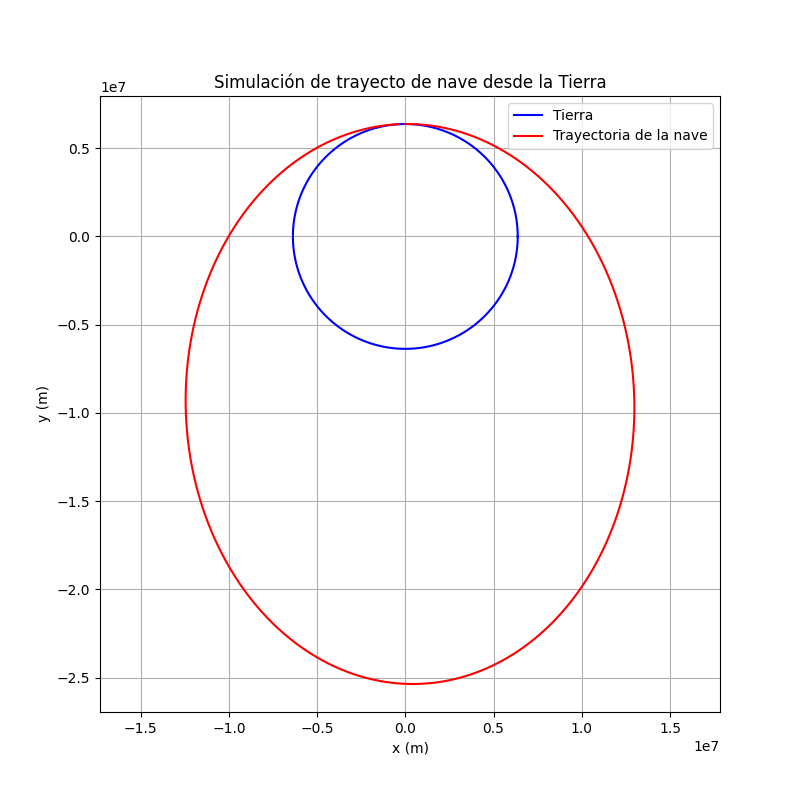
\includegraphics[width=0.8\textwidth]{img/3.png}
    \caption{Movimiento de 2 cuerpos: Trayectoria de la nave espacial}
    \label{fig:salida_consola}
\end{figure}

	\subsubsection{Análisis de órbita espacial}
	
	\textbf{Caso suborbital ($v_0 < v_{escape}$):}
	implementa una simulación numérica del movimiento de una nave espacial bajo la influencia gravitacional de la Tierra utilizando el método de Euler. Permite analizar la trayectoria de la nave  y visualizar la órbita según la energía específica del sistema.

	\subsection{Problema 4: Movimiento de 2 cuerpos}
	
	\subsubsection{Formulación del problema de N-cuerpos}
	
	El problema de N-cuerpos consiste en resolver el sistema de ecuaciones diferenciales:
	
	\begin{equation}
		\frac{d^2\mathbf{r}_i}{dt^2} = \sum_{j=1, j \neq i}^{N} \frac{Gm_j(\mathbf{r}_j - \mathbf{r}_i)}{|\mathbf{r}_j - \mathbf{r}_i|^3}
	\end{equation}
	
	para $i = 1, 2, \ldots, N$.
	
	\textbf{Características del sistema de 4 cuerpos:}
	\begin{itemize}
	\item Sistema no integrable analíticamente (para N ≥ 3)
	\item Comportamiento potencialmente caótico
	\item Conservación de energía, momento lineal y angular
	\item Sensibilidad a condiciones iniciales
	\end{itemize}
	
	\subsubsection{Implementación numérica avanzada}
	
	\begin{lstlisting}[language=Python, caption={Sistema completo de 4 cuerpos con análisis dinámico}]
import numpy as np
import matplotlib.pyplot as plt

def aceleracion(x1, y1, x2, y2, suave=0.001):
    dx = x1 - x2
    dy = y1 - y2
    r = np.sqrt(dx**2 + dy**2)
    if r == 0:
        return 0, 0
    factor = -1 / (r**3 + suave)
    return dx * factor, dy * factor


def main():
    # constantes
    cuerpos = [
        (2,3),
        (-1,-1),
        (3,-0.5)
    ]

    r = 1
    limit = 8

    # Graficar circunferencia 1
    theta = np.linspace(0, 2 * np.pi, 100)

    for i, (x, y) in enumerate(cuerpos):
        x1 = x + r * np.cos(theta)
        y1 = y + r * np.sin(theta)

        # Graficar circunferencia
        plt.plot(x1, y1, label=f'Cuerpo {i+1}')

    # Párametros para la simulación
    h = 0.01
    tfin = 100
    
    for vy0 in np.arange(0.9, 1.5, 0.05):
        vy = vy0
        vx = -0.45
        y = 1
        x = 0

        px = [x]
        py = [y]

        graficar = True

        for _ in np.arange(0, tfin, h):
            x = x + vx * h
            y = y + vy * h

            ax_total, ay_total = 0, 0

            for x1, y1 in cuerpos:
                # Calcular aceleración
                ax, ay = aceleracion(x, y, x1, y1)
                ax_total += ax
                ay_total += ay
            
            vx = vx + ax_total * h
            vy = vy + ay_total * h

            # Verificar límites
            if x > limit or x < -limit or y > limit or y < -limit:
                graficar = False
                break

            # Verificar colisión con los círculos
            stop = False
            for x1, y1 in cuerpos:
                if ((x - x1)**2 + (y - y1)**2) <= r**2:
                    stop = True

            if stop:
                break

            px.append(x)
            py.append(y)


        if graficar:
            plt.plot(px, py, label=f'Trajectoria (vy={vy0:.2f})')

    # Configuracion del gráfico
    plt.axis('equal')
    plt.grid(True)
    plt.xlabel('x')
    plt.ylabel('y')
    plt.xlim(-limit, limit)
    plt.ylim(-limit, limit)
    plt.axhline(0, color='black', lw=1, label='Eje X', linestyle='--')
    plt.axvline(0, color='black', lw=1, label='Eje Y', linestyle='--')
    plt.gca().set_aspect('equal', adjustable='box')
    plt.title('Trayectorias de partículas')
    plt.legend()
    plt.show()

if __name__ == "__main__":
    main()
	\end{lstlisting}

	\begin{figure}[H]
    \centering
    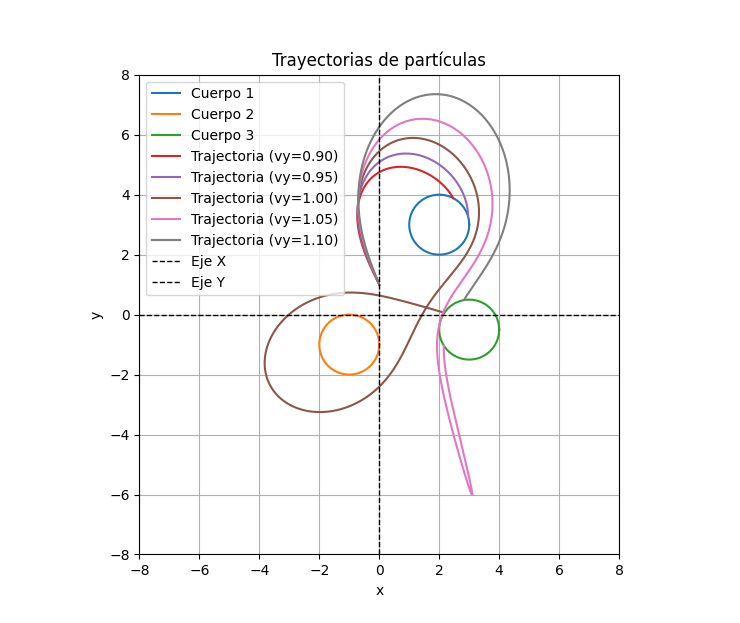
\includegraphics[width=0.8\textwidth]{img/4.png}
    \caption{Movimiento de 4 cuerpos: Trayectorias de partículas}
    \label{fig:salida_consola}
\end{figure}
    
    \subsubsection{Análisis de la trayectoria de la partícula}

El código simula la trayectoria de una partícula bajo la influencia de varios cuerpos fijos, utilizando una integración numérica mediante el método de Euler. Cada cuerpo genera una atracción análoga a una fuerza gravitacional suavizada para evitar singularidades. Se estudia cómo varía la trayectoria de la partícula al modificar su velocidad inicial vertical.

\textbf{Criterios de estabilidad:}
\begin{itemize}
\item \textbf{Conservación aproximada de energía:} Aunque el método de Euler no conserva exactamente la energía, se analiza la estabilidad cualitativa de la trayectoria.
\item \textbf{Acotamiento de las órbitas:} Se considera estable una trayectoria si permanece dentro de una región limitada del espacio.
\item \textbf{Ausencia de colisiones o escapes:} Se evalúa si la partícula evita colisionar con los cuerpos fijos o salir del dominio simulado.
\end{itemize}

\textbf{Indicadores de comportamiento caótico:}
\begin{itemize}
\item \textbf{Sensibilidad a condiciones iniciales:} Pequeñas variaciones en la velocidad inicial producen trayectorias marcadamente diferentes.
\item \textbf{Divergencia rápida de trayectorias:} Se observa la separación entre trayectorias que parten de estados casi idénticos.
\item \textbf{Complejidad estructural de las trayectorias:} La geometría irregular y no periódica sugiere un sistema caótico, especialmente en presencia de múltiples atractores.
\end{itemize}

	\subsection{Problema 5: Movimiento oscilatorio -- Figuras de Lissajous 3D}
	
	\subsubsection{Fundamentos teóricos}
	
	Las figuras de Lissajous son curvas paramétricas que resultan de la superposición de movimientos armónicos simples en diferentes direcciones:
	
	\begin{align}
		x(t) &= A_1 \sin(\omega_1 t + \phi_1) \\
		y(t) &= A_2 \sin(\omega_2 t + \phi_2) \\
		z(t) &= A_3 \sin(\omega_3 t + \phi_3)
	\end{align}
	
	\textbf{Parámetros característicos:}
	\begin{itemize}
	\item $A_i$: Amplitudes de oscilación
	\item $\omega_i$: Frecuencias angulares
	\item $\phi_i$: Fases iniciales
	\end{itemize}
	
	\textbf{Propiedades importantes:}
	\begin{itemize}
	\item Si $\omega_1/\omega_2$ es racional, la curva es cerrada (periódica)
	\item Si $\omega_1/\omega_2$ es irracional, la curva llena densamente una región
	\item La diferencia de fase determina la orientación de la figura
	\end{itemize}

	\subsubsection{Extensión a osciladores acoplados}
	
	Para osciladores acoplados en 3D, el sistema de ecuaciones es:
	
	\begin{align}
		\frac{d^2x}{dt^2} &= -\omega_1^2 x + \gamma(y - x) + \gamma(z - x) \\
		\frac{d^2y}{dt^2} &= -\omega_2^2 y + \gamma(x - y) + \gamma(z - y) \\
		\frac{d^2z}{dt^2} &= -\omega_3^2 z + \gamma(x - z) + \gamma(y - z)
	\end{align}
	
	donde $\gamma$ es la constante de acoplamiento.

	\begin{lstlisting}[language=Python, caption={Análisis completo de figuras de Lissajous 3D y osciladores acoplados}]
import numpy as np
import matplotlib.pyplot as plt

# Parámetros
l = 2
n = 3
o = 6

k1, m1 = l**2, 1
k2, m2 = n**2, 1
k3, m3 = o**2, 1

# Condiciones iniciales
x, vx = 1, 2.36
y, vy = 1, 2.36
z, vz = 1, 2.36

# Tiempo de simulación
h = 0.01
tfin = 50
t = np.arange(0, tfin + h, h)

# Inicialización
px = np.zeros_like(t)
py = np.zeros_like(t)
pz = np.zeros_like(t)
px[0], py[0], pz[0] = x, y, z

# Simulación con método de Euler
for i in range(len(t)):
    ax = -k1/m1 * x
    ay = -k2/m2 * y
    az = -k3/m3 * z

    vx += h * ax
    vy += h * ay
    vz += h * az

    x += h * vx
    y += h * vy
    z += h * vz

    px[i] = x
    py[i] = y
    pz[i] = z

# Gráficos
fig = plt.figure(figsize=(12, 10))

# Subplot 3D
ax1 = fig.add_subplot(2, 2, 1, projection='3d')
ax1.plot(px, py, pz, color='brown')
ax1.set_title(f'Lissajous 3D: l={l}, n={n}, z={o}')
ax1.set_xlabel('x')
ax1.set_ylabel('y')
ax1.set_zlabel('z')

# Subplot XY
ax2 = fig.add_subplot(2, 2, 2)
ax2.plot(px, py, color='red')
ax2.set_title(f'Plano XY (l={l}, n={n})')
ax2.set_xlabel('x')
ax2.set_ylabel('y')
ax2.axis('equal')
ax2.grid(True)

# Subplot XZ
ax3 = fig.add_subplot(2, 2, 3)
ax3.plot(px, pz, color='green')
ax3.set_title(f'Plano XZ (l={l}, o={o})')
ax3.set_xlabel('x')
ax3.set_ylabel('z')
ax3.axis('equal')
ax3.grid(True)

# Subplot YZ
ax4 = fig.add_subplot(2, 2, 4)
ax4.plot(py, pz, color='blue')
ax4.set_title(f'Plano YZ (n={n}, o={o})')
ax4.set_xlabel('y')
ax4.set_ylabel('z')
ax4.axis('equal')
ax4.grid(True)

plt.tight_layout()
plt.show()
	\end{lstlisting}

    \begin{figure}[H]
    \centering
    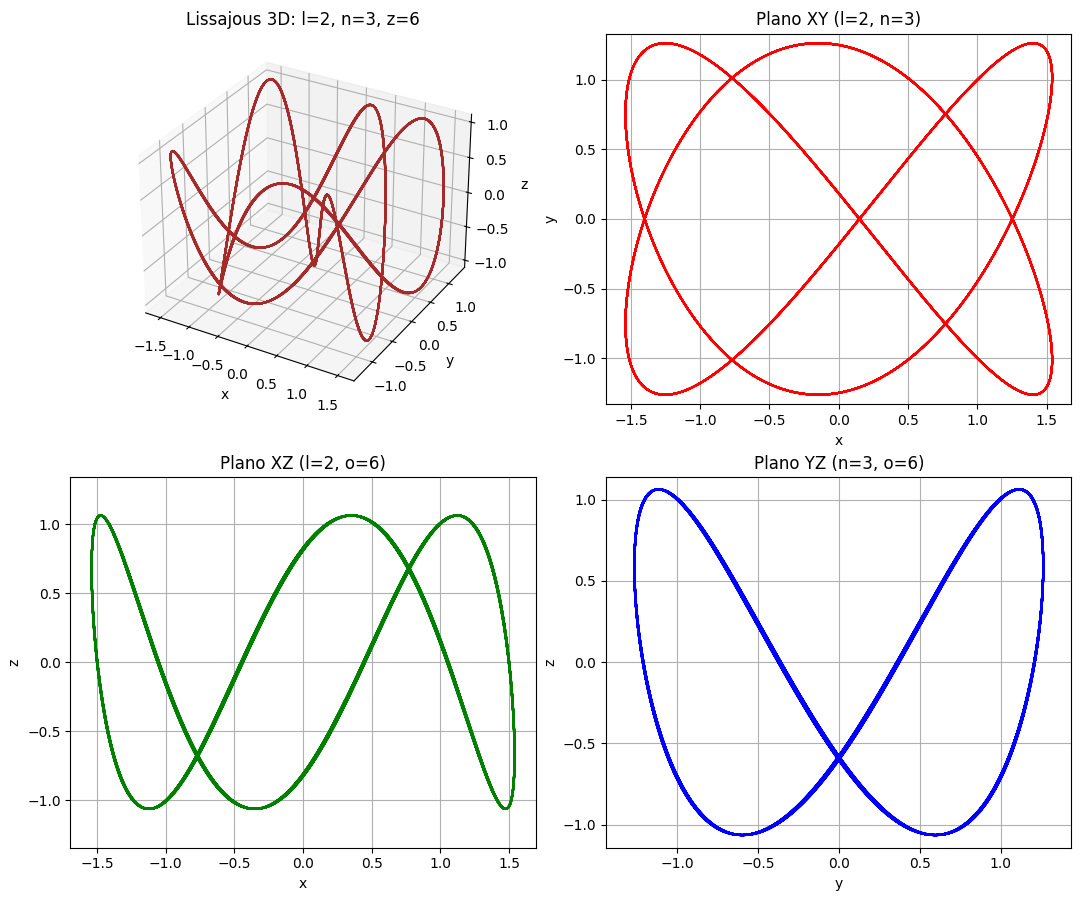
\includegraphics[width=0.8\textwidth]{img/5.png}
    \caption{Movimiento de 4 cuerpos: Trayectorias de partículas}
    \label{fig:salida_consola}
\end{figure}

	\subsubsection{Análisis de oscilaciones tridimensionales acopladas}
Este código simula un sistema de osciladores armónicos simples en tres dimensiones, donde cada coordenada x,y,zx, y, zx,y,z está sujeta a una fuerza restauradora proporcional a su desplazamiento, lo que da lugar a trayectorias del tipo de curvas de Lissajous en 3D. La integración se realiza mediante el método de Euler explícito.
\textbf{Características del sistema:}
\begin{itemize}
\item \textbf{Osciladores independientes:} Cada eje presenta un movimiento armónico simple con constante elástica k=ω2=l2,n2,o2k = \omega^2 = l^2, n^2, o^2k=ω2=l2,n2,o2 y masa m=1m = 1m=1.
\item \textbf{Trayectoria en el espacio tridimensional:} La combinación de tres frecuencias distintas produce curvas complejas en el espacio.
\item \textbf{Condiciones iniciales iguales:} Las posiciones y velocidades iniciales son iguales en los tres ejes, lo que induce simetría en la evolución inicial.
\end{itemize}
\textbf{Interpretación de la figura generada:}
\begin{itemize}
\item \textbf{Gráfico 3D:} La trayectoria espaciotemporal representa una curva de Lissajous tridimensional, resultado de la superposición de tres oscilaciones sinusoidales con frecuencias racionalmente relacionadas.
\item \textbf{Proyecciones 2D:} Las gráficas en los planos XY, XZ y YZ permiten analizar la relación de fase entre los pares de componentes, revelando patrones de interferencia o resonancia.
\end{itemize}
\textbf{Aplicaciones:}
\begin{itemize}
\item Visualización de modos normales en sistemas oscilatorios.
\item Análisis de sistemas lineales desacoplados en física clásica o mecánica cuántica.
\item Demostración de la formación de patrones en sistemas dinámicos tridimensionales.
\end{itemize}

    \section{Conclusiones}
En este trabajo se ha estudiado la resolución numérica de sistemas de ecuaciones diferenciales ordinarias (EDOs) utilizando el método de Euler, aplicándolo a una variedad de modelos físicos que incluyen trayectorias gravitacionales, oscilaciones armónicas y movimientos tridimensionales acoplados. Los resultados obtenidos permiten extraer las siguientes conclusiones:
\begin{itemize}
\item \textbf{Precisión y convergencia:} El método de Euler, de orden de convergencia p=1p = 1p=1, demuestra una precisión limitada que mejora al reducir el tamaño del paso hhh, aunque esto incrementa significativamente el tiempo de cómputo. Su simplicidad lo hace útil para análisis cualitativos o como base para métodos más avanzados.
\item \textbf{Comportamiento no lineal y caos:} En la simulación del problema de N-cuerpos se evidencia una marcada sensibilidad a las condiciones iniciales. Esta propiedad, junto con la divergencia de trayectorias cercanas y la complejidad de los patrones obtenidos, sugiere la presencia de comportamiento caótico, típico de sistemas dinámicos no lineales.
\item \textbf{Representación visual del sistema dinámico:} Las trayectorias obtenidas —como las órbitas de interacción gravitacional y las curvas de Lissajous en 3D— permiten una visualización clara e intuitiva de los fenómenos simulados. Esto facilita la comprensión de las dinámicas acopladas y de la evolución temporal de sistemas multivariables.
\end{itemize}
En conjunto, estos hallazgos refuerzan el valor pedagógico y práctico del método de Euler como herramienta básica para la exploración numérica de sistemas físicos complejos, proporcionando una puerta de entrada accesible al análisis computacional de la dinámica clásica.

    \end{document}
